\section{Results}
\label{sec:results}

For evaluating our dataset generation, we first collected commits without any limits imposed on commits from a single author. We later added a per-author limit in order to avoid bias being introduced by including a vast amount of commits from a single author.

\autoref{fig:total_vs_tagged_with_limit} shows that around 25000 commits (~2.5\%) out of a total of 1000000 commits are tagged when limiting the number of commits per author to 100. Without this limit, the number of tagged commits slightly increases to about 35000 commits (~3.5\%) out of 1000000. Overall, we see that with or without limit, the number of tagged commits remains relatively small compared to the total number of commits.

\begin{figure}[H]
  \centering
  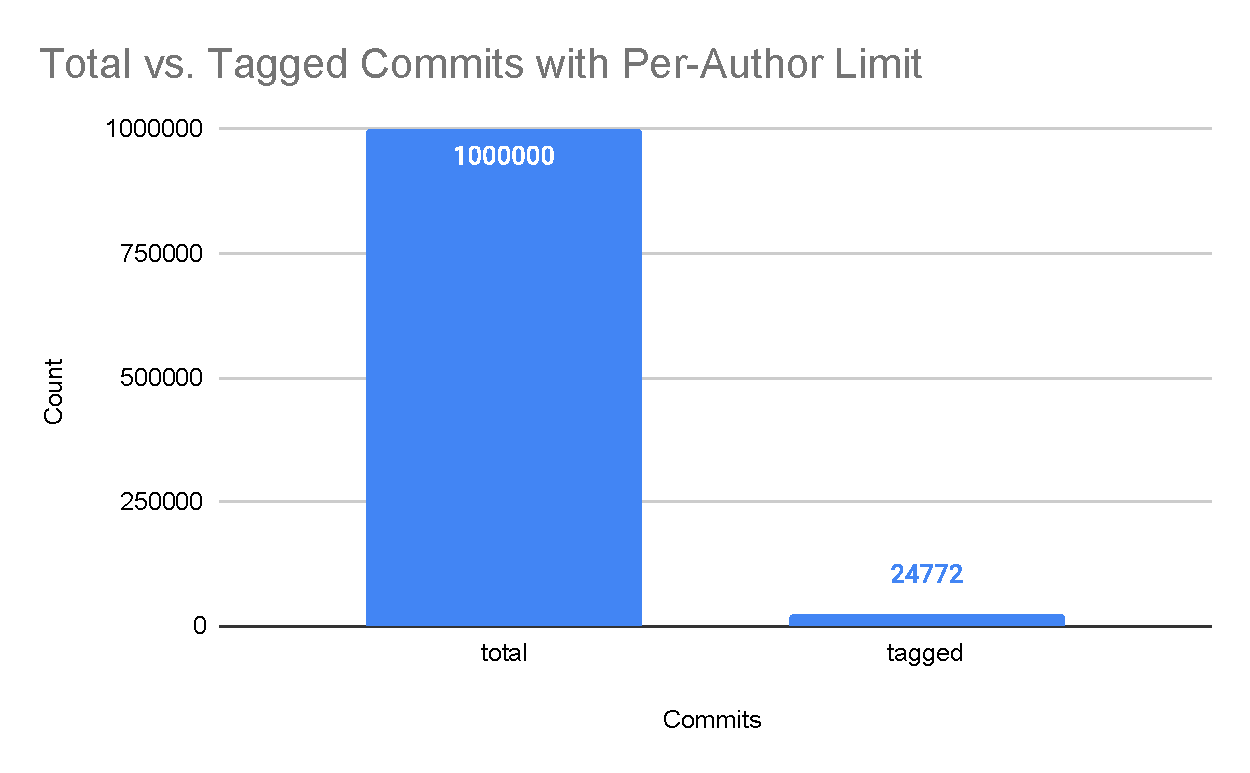
\includegraphics[width=\textwidth]{total-vs-tagged-commits-with-author-limit.pdf}
  \caption{Total vs. Tagged Commits with Per-Author Limit}
  \label{fig:total_vs_tagged_with_limit}
\end{figure}

\begin{figure}[H]
  \centering
  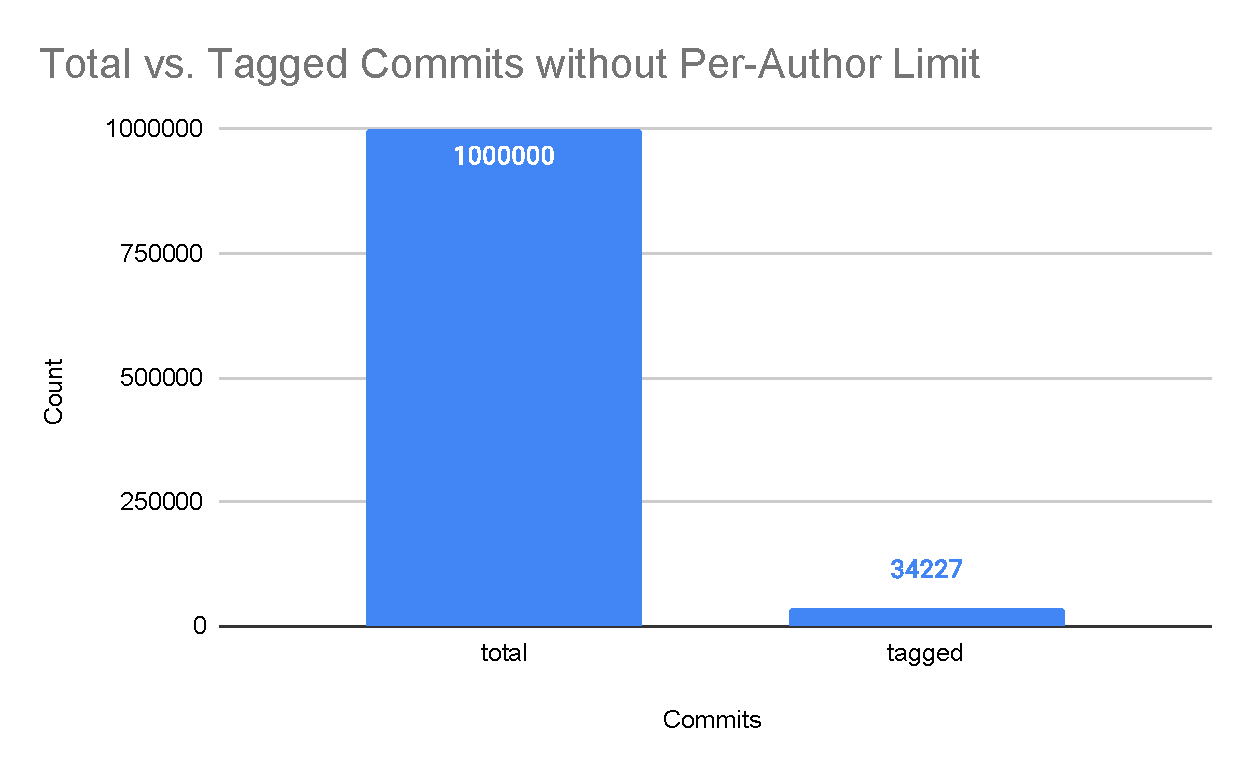
\includegraphics[width=\textwidth]{total-vs-tagged-commits-without-author-limit.pdf}
  \caption{Total vs. Tagged Commits without Per-Author Limit}
  \label{fig:total_vs_tagged_without_limit}
\end{figure}

In \autoref{fig:tag_dist_with_limit} and \autoref{fig:tag_dist_without_limit}, we can see the distribution of commit tags with and without the mentioned per-author limit, respectively. When comparing both graphs, we can see that without a per-author commit limit, the number of commits tagged with “chore” almost doubles while commits tagged with “feat” stay more or less the same. This is likely due to commits being authored by bots, which mainly applies to automatic maintenance tasks, i.e. chores.

\begin{figure}[H]
  \centering
  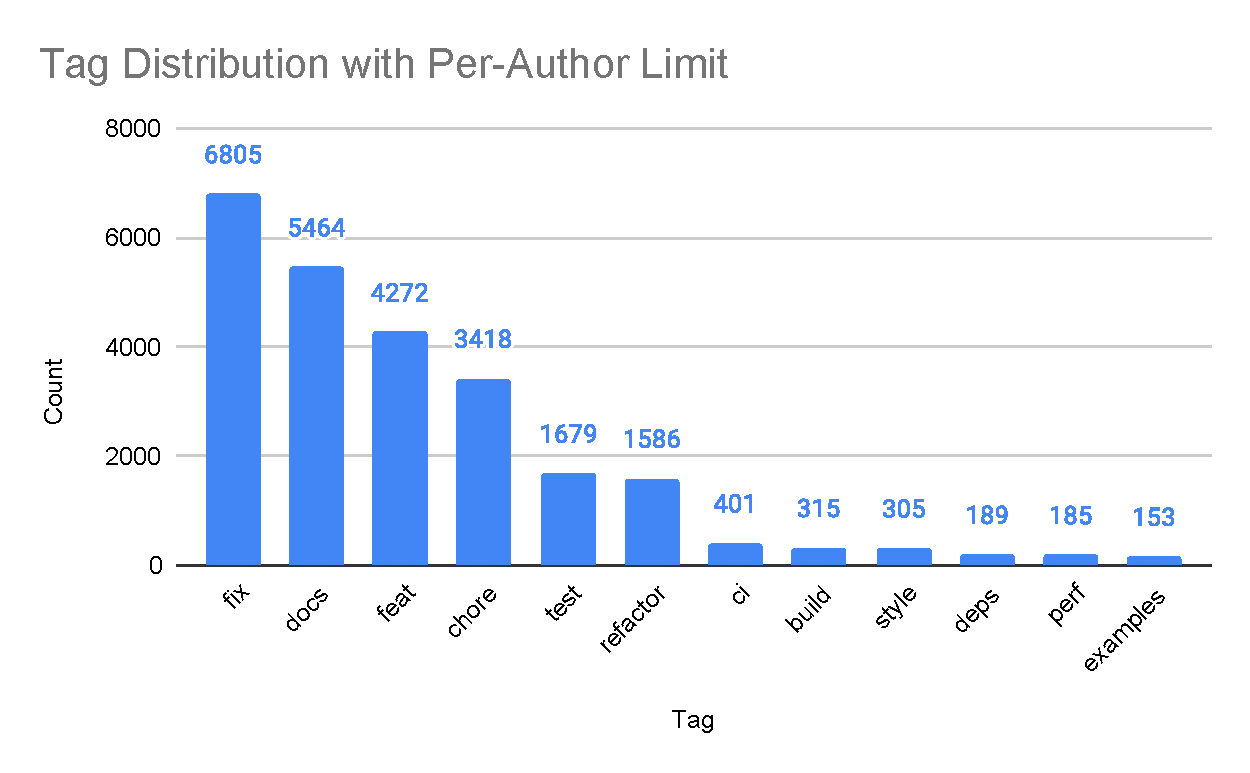
\includegraphics[width=\textwidth]{tag-distribution-with-author-limit.pdf}
  \caption{Tag Distribution with Per-Author Limit}
  \label{fig:tag_dist_with_limit}
\end{figure}

\begin{figure}[H]
  \centering
  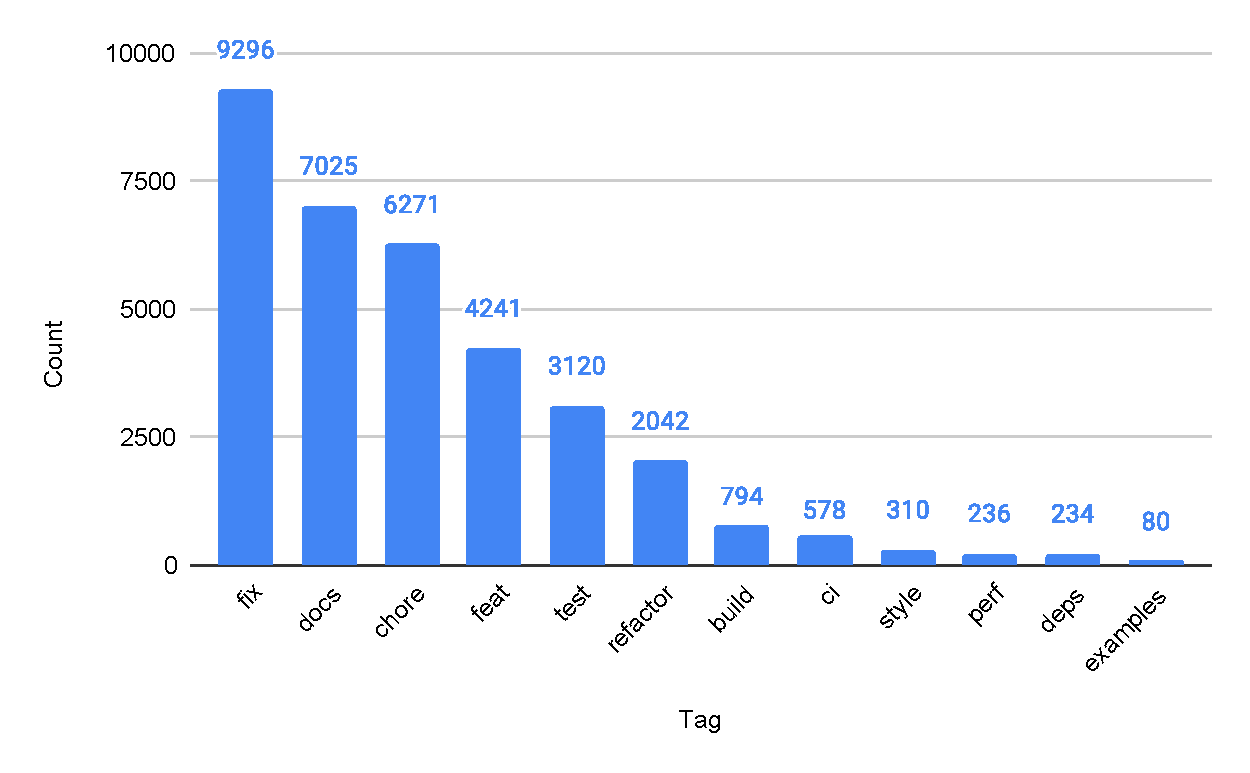
\includegraphics[width=\textwidth]{tag-distribution-without-author-limit.pdf}
  \caption{Tag Distribution without Per-Author Limit}
  \label{fig:tag_dist_without_limit}
\end{figure}

\begin{table}[H]
  \def\arraystretch{1.15}%
  \centering
  \caption{Unlimited commit messages per author}
  \bigskip
  \begin{tabular}{| l | r |}
    \hline
    Total Accuracy & 0.6517433833828978 \\
    \hline
    Total F1 micro & 0.6517433833828978 \\
    \hline
    Total F1 macro & 0.5371101432803524 \\
    \hline
  \end{tabular}
\end{table}

\begin{table}[H]
  \def\arraystretch{1.15}%
  \centering
  \caption{100 commit messages per author}
  \bigskip
  \begin{tabular}{| l | r |}
    \hline
    Total Accuracy & 0.6102058422223566 \\
    \hline
    Total F1 micro & 0.6102058422223566 \\
    \hline
    Total F1 macro & 0.4479298698746271 \\
    \hline
  \end{tabular}
\end{table}

